\chapter{Contexte général du projet}
\label{chap:Contexte général du projet}



Dans ce chapitre, nous situons notre stage de fin d’études dans son environnement organisationnel et contextuel. Nous présentons l’organisme d’accueil 4D logiciel. Ensuite nous expliquons la méthodologie adoptée durant la réalisation de notre projet ainsi que sa planification.

\newpage


\section{Pésentation de l’organisme d’accueil}

\begin{figure}[h]
    \centering
    
\includegraphics[scale=0.5]{Logos/Logo-4D.jpg} % Replace with the actual filename of the IBM logo image
    \caption{Logo 4D }
    \label{fig:Logo4D}
\end{figure}

Fondée en 1984 par Laurent Ribardière, 4D Logiciels est une entreprise de conseil et de développement de logiciels dans le domaine des systèmes d’information, de l’organisation et de l’informatique, dont le siège social se situe à Clichy (Île-de-France). Ribardière a créé 4D avec une seule ambition : simplifier la création des applications professionnelles pour les entreprises grâce à une base de données relationnelles entièrement graphique. 4D est ainsi devenue l’un des premiers éditeurs de logiciels français avec un rayonnement international, grâce à sa présence sur les cinq continents et des filiales dans plus de dix pays, dont le Maroc (4D Logiciels Maroc). Son succès vient de sa capacité à répondre aux enjeux de son époque grâce à une plateforme évolutive, facilitant la création d’expériences clients réussies sur mobile, web et desktop. \cite{ref1}

%%%%%%%%%%%%%%%%%%%% subsection 1 %%%%%%%%%%%%%%%%%%%%%%%

\subsection{Histoire de 4D}


\begin{figure}[h]
    \centering
    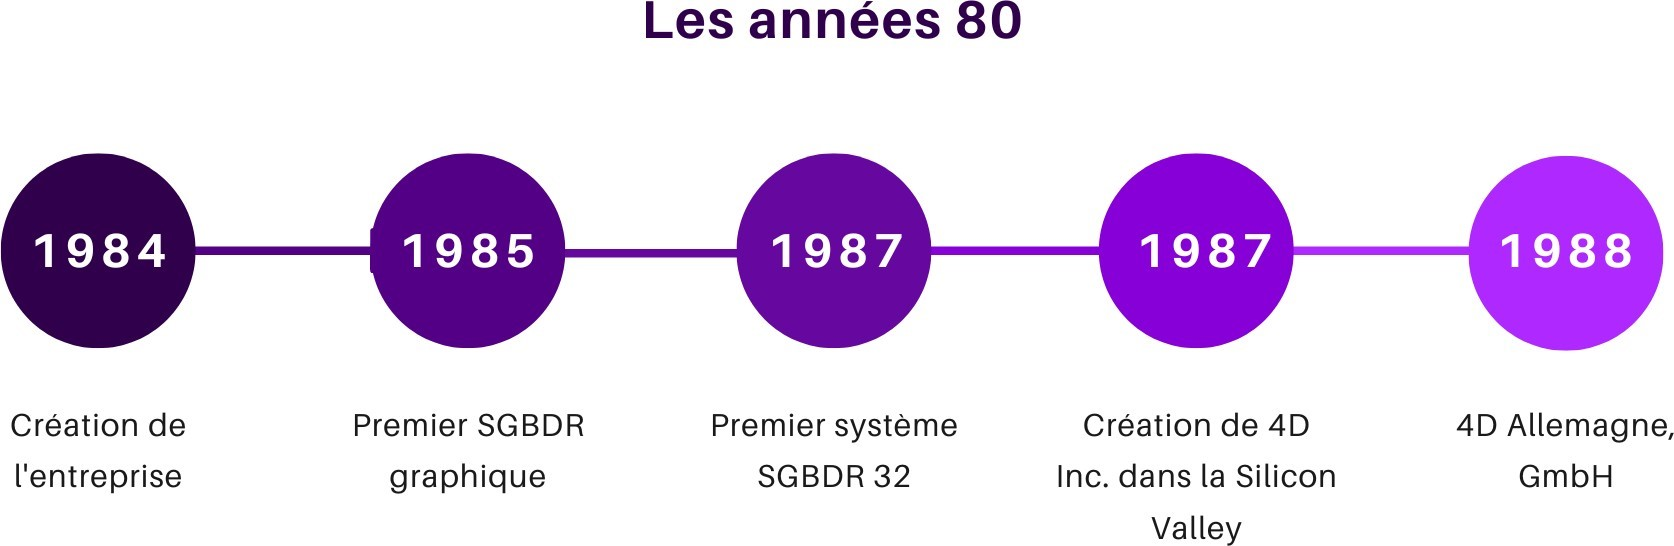
\includegraphics[scale=0.3]{Figures/80.jpg} % Replace with the actual filename of the IBM logo image
    \caption{Les années 80 \cite{4Dhistory}}
    \label{fig:Histoire80}
\end{figure}


En 1987 , 4D Logiciels propose le premier système de gestion de base de données relationnel fonctionnant sur un système 32-bits, puis conserve sa place de leader en offrant le premier :
\begin{itemize}
    \item[$\bullet$]  Client-serveur intégré.
    \item[$\bullet$]  Serveur web intégré.
    \item[$\bullet$]  Système de partage d’applications dynamique intégré.
\end{itemize}
\vspace{1cm}

\begin{figure}[h]
    \centering
    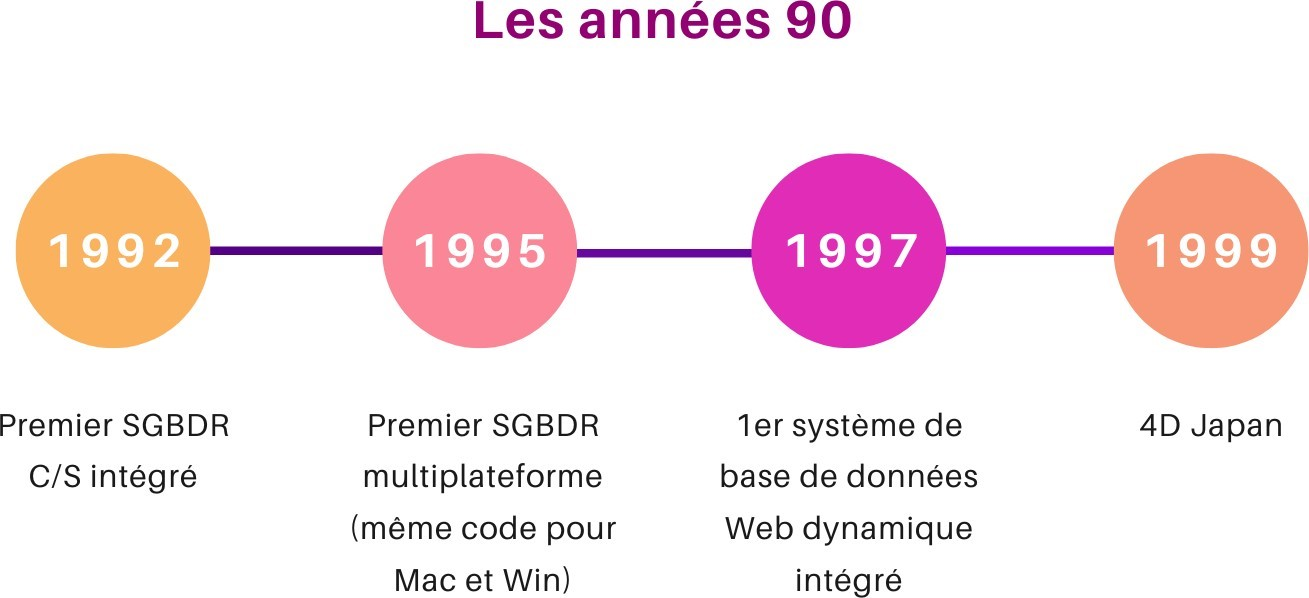
\includegraphics[scale=0.3]{Figures/90.jpg} % Replace with the actual filename of the IBM logo image
    \caption{Les années 90 \cite{4Dhistory}}
    \label{fig:Histoire90}
\end{figure}
% \vspace{lcm}

En 1997, 4D décide de s’investir dans le Web en donnant lieu 
à un serveur Web dynamique. Ce qui aide les développeurs à servir
à la fois des applications client-serveur et des applications
Web sans modifier le code. 4D conserve par la suite ce produit 
en lançant à chaque fois des nouvelles versions.

\begin{figure}[h]
    \centering
    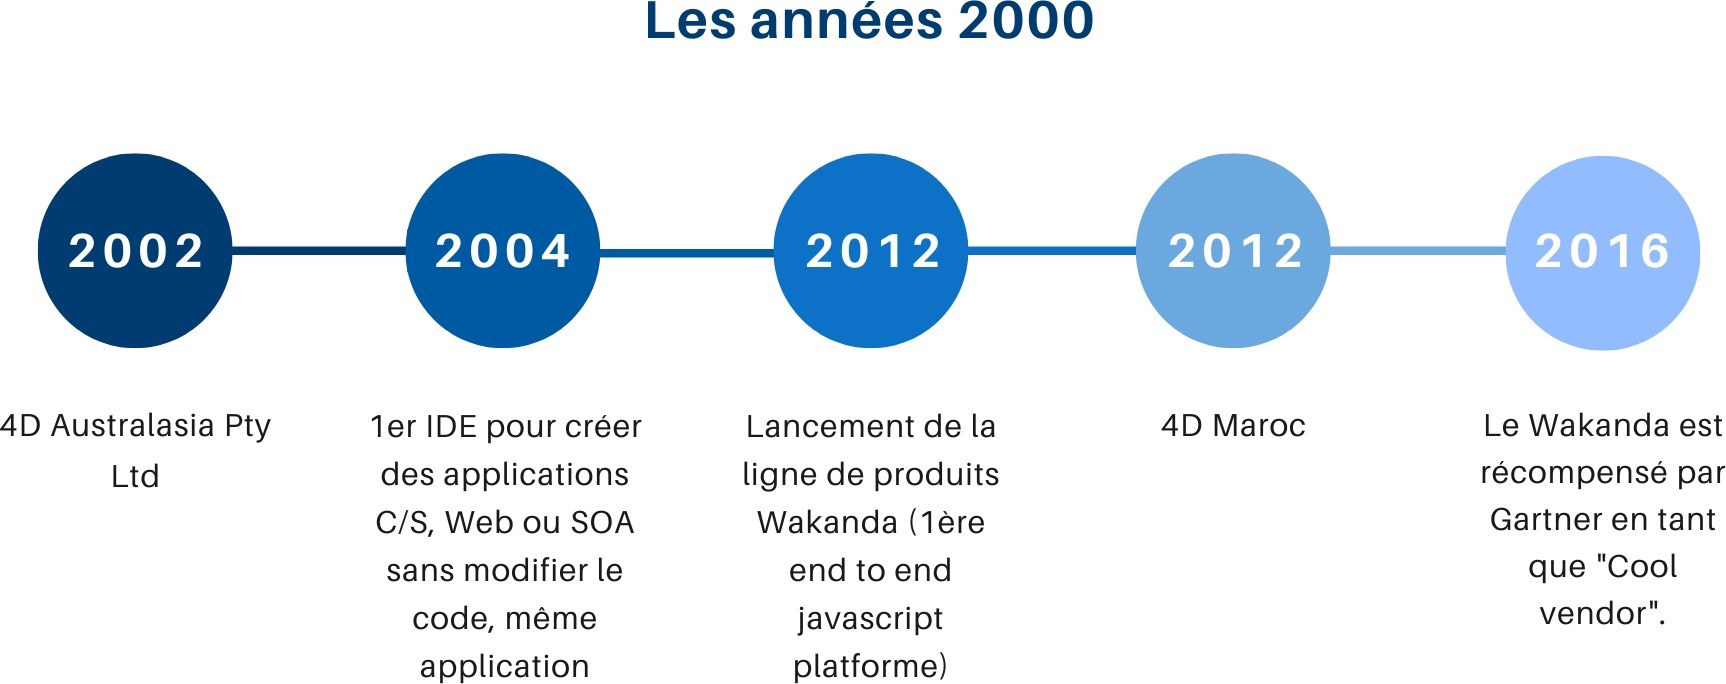
\includegraphics[scale=0.3]{Figures/20.jpg} % Replace with the actual filename of the IBM logo image
    \caption{Les années 2000 \cite{4Dhistory}}
    \label{fig:Histoire90}
\end{figure}

La version 4D 2004 se lance en tant qu’un produit permettant aux développeurs 
de créer à la fois des applications autonomes, client-serveur, Web, 
ainsi que des applications orientées Services (SOA) sans rajouter 
aucun changement au niveau du code.
Plus récemment, 4D dispose d’une plateforme de développement 
en JavaScript qui facilite la création des applications 
professionnelles en utilisant la gamme de produits Wakanda.


%%%%%%%%%%%%%%%%%%%% subsection 2 %%%%%%%%%%%%%%%%%%%%%%%

%%%%%%%%%%%%%%%%%%%% subsection 3 %%%%%%%%%%%%%%%%%%%%%%%

\subsection{La structure du groupe 4D}

Le groupe 4D est composé d’un siège social situé en France, 
et de cinq filiales situées aux États-Unis, en Allemagne, 
en Australie, au Japon, et au Maroc. À l’écoute permanent 
de leurs besoins et des évolutions technologiques, 
la société offre une expérience enrichissante dans un contexte multiculturel grâce à ses différentes implantations internationales (Sydney, Tokyo, San José, Munich, Rabat).

\vspace{1cm}

\begin{figure}[h]
    \centering
    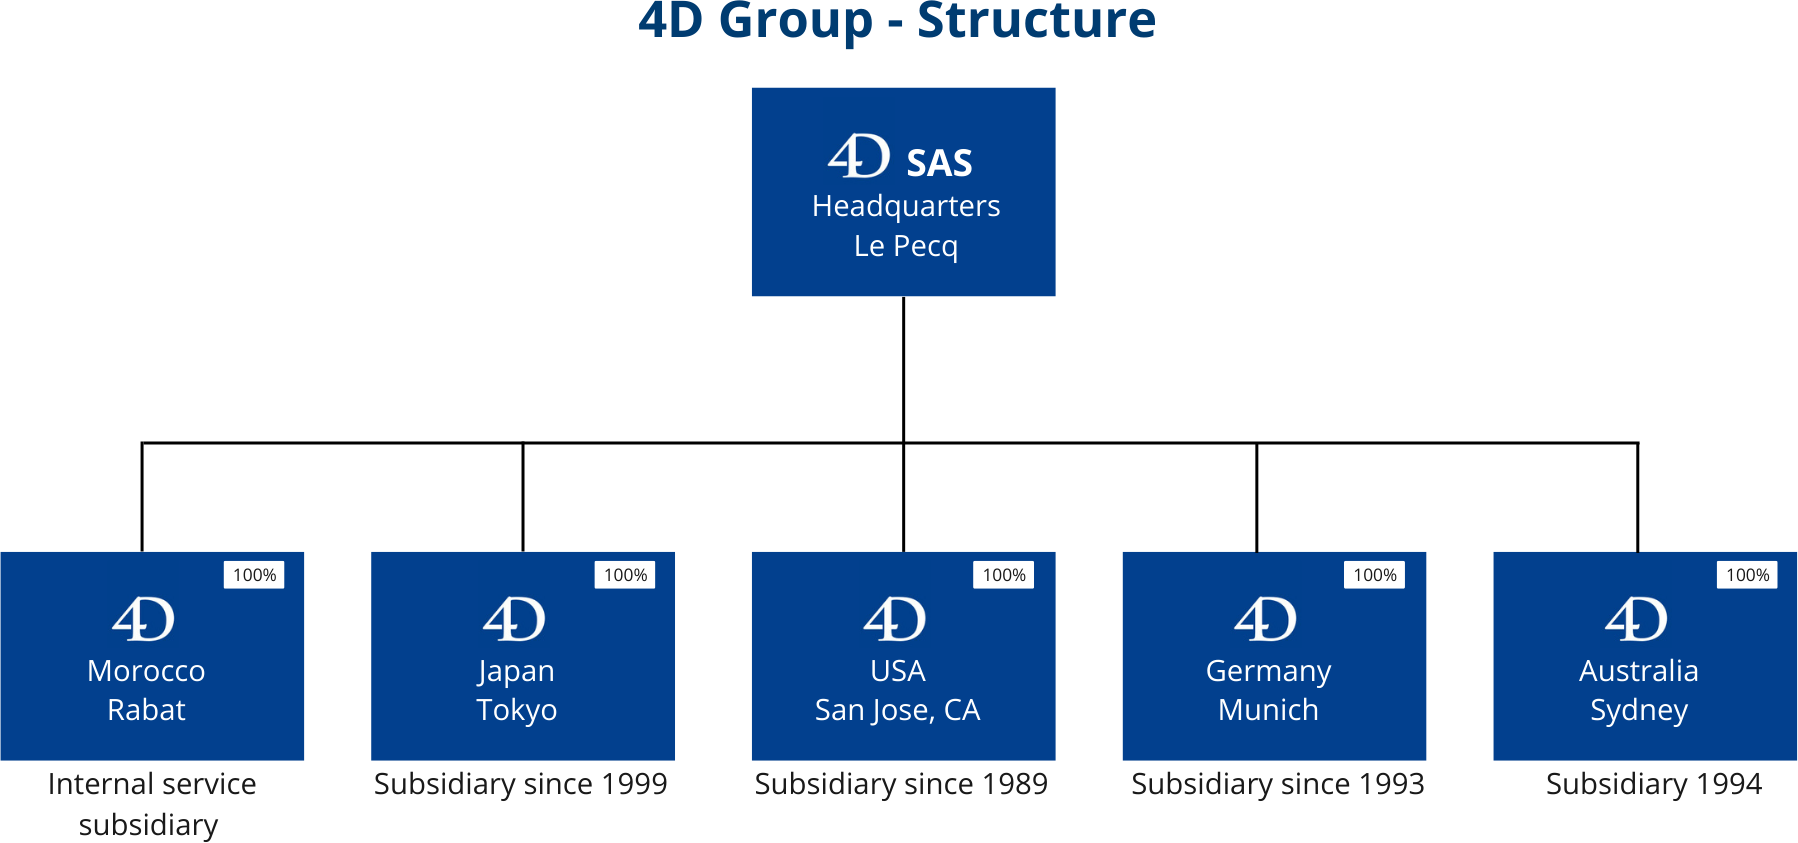
\includegraphics[scale=0.35]{Figures/groupe.png} % Replace with the actual filename of the IBM logo image
    \caption{Le groupe 4D dans le monde}
    \label{fig:groupe}
\end{figure}

Comme toute société renommée, 4D recourt à ses différents partenaires 
pour un rendu meilleur et un niveau d’expertise plus crédible. 4D connaît aussi 
une présence internationale grâce à ses partenaires et ses distributeurs éparpillés 
dans le monde, comme montre la figure suivante :

\begin{figure}[h]
    \centering
    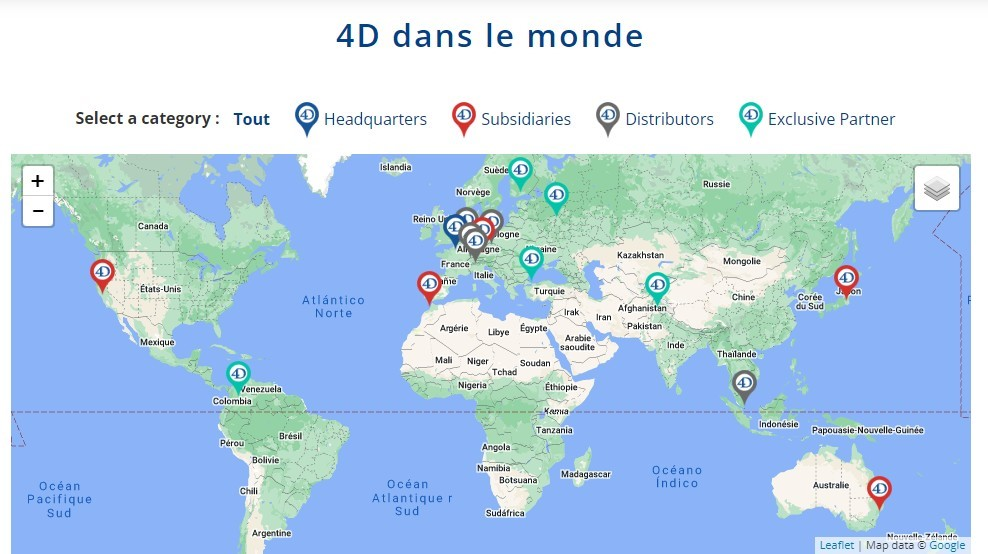
\includegraphics[scale=0.6]{Figures/carte.jpg} % Replace with the actual filename of the IBM logo image
    \caption{Les points de présence des partenaires et des distributeurs de 4D \cite{4Dhistory}}
    \label{fig:carte}
\end{figure}

\vspace{6cm}

La figure ci-dessous montre la direction générale de l’entreprise 4D logiciels :



\begin{figure}[h]
    \centering
    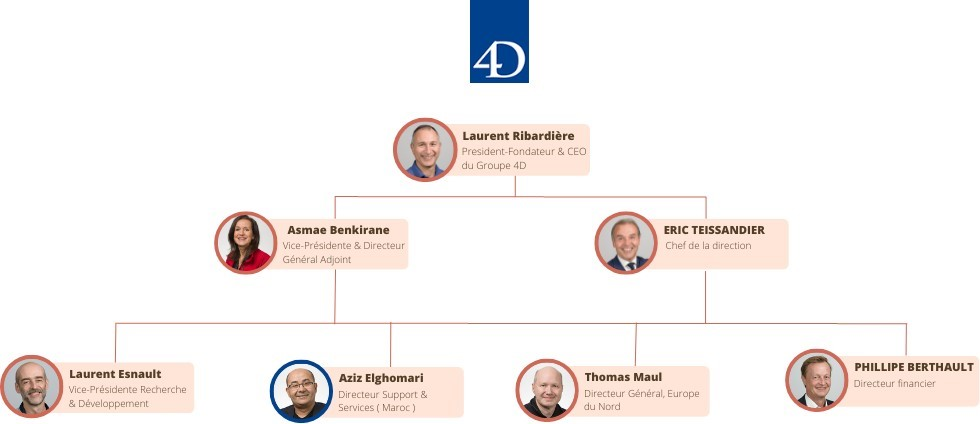
\includegraphics[scale=0.6]{Figures/direction.jpg} % Replace with the actual filename of the IBM logo image
    \caption{La Direction Générale de 4D}
    \label{fig:direction}
\end{figure}

%%%%%%%%%%%%%%%%%%%% subsection 4 %%%%%%%%%%%%%%%%%%%%%%%
\subsection{Les domaines métiers et les clients 4D}
4D intervient dans une diversité de domaines, comme 
la santé, l’éducation, l’administration, la gouvernance, 
et les télécommunications. La figure 1.8 montre le pourcentage 
qu’occupe chaque domaine dans son activité.

\begin{figure}[h]
    \centering
    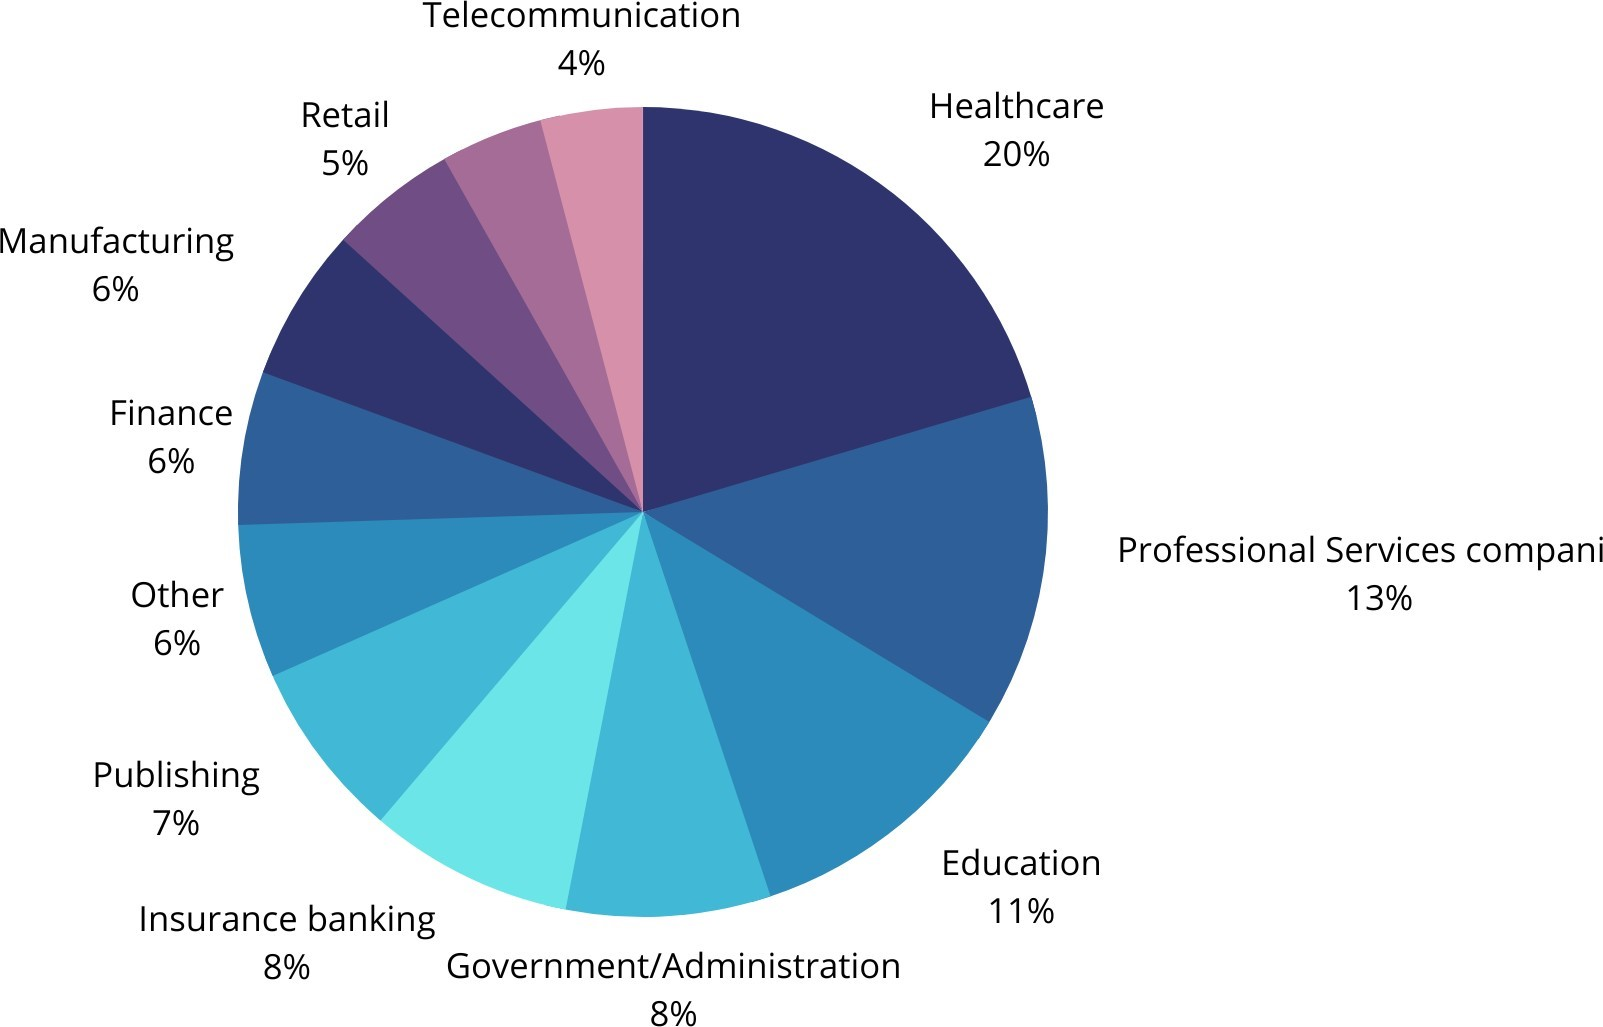
\includegraphics[scale=0.7]{Figures/domaineMetier.jpg} % Replace with the actual filename of the IBM logo image
    \caption{Les domaines métiers de 4D en pourcentage}
    \label{fig:domaineMetier}
\end{figure}


%%%%%%%%%%%%%%%%%%%% SECTION 3 %%%%%%%%%%%%%%%%%%%%%%%


\subsection{Le Langage 4D}

4D est une plateforme de développement productive qui permet aux clients
 de se concentrer sur leur modèle de données et les règles 
 et spécificités de leur métier \cite{ref1}.

 4D Serveur exécute leurs applications simultanément sur les postes de travail
/ clients mobiles et sur le Web. Ils peuvent déployer des applications 
entièrement personnalisées sous leur propre marque.
 4D est un système de gestion de base de données 
 relationnelle disposant d’un langage de programmation 
 de la quatrième génération.

Environnement de développement intégré, 4D intègre :
\begin{itemize}
    \item un compilateur;
    \item un débogueur;
    \item un système de sauvegarde et de réplication;
    \item un serveur Web;
    \item un serveur et client de services web.
\end{itemize}


4D v18 marque un véritable tournant dans l’histoire de 4D. Cette version propose non seulement de
multiples nouvelles fonctionnalités, mais aussi l’amélioration de fonctions existantes. Elle introduit la gestion de version pour changer 
la façon dont les équipes collaborent. Le format texte des bases projets permet désormais de tirer pleinement parti des systèmes de gestion de version
(par exemple, Git, SVN, etc.). Autre fonctionnalité qui fait ses débuts dans cette nouvelle version : une solution intégrée de chiffrement des données, 
offrant en un seul clic une sécurité maximum aux données des clients. Ces outils de chiffrement sont basés sur l’un des algorithmes les plus sûrs : 
Advanced Encryption Standard (AES). ORDA (Object Relational Data Access), la technologie révolutionnaire d’accès et de présentation 
des données, apporte également son lot de nouvelles fonctionnalités, telles que le Datastore distant, ouvrant de nouvelles perspectives et optimisant les 
performances du client/serveur. Les applications métiers peuvent facilement être déployées sur des appareils mobiles avec 4D for iOS, une solution 
entièrement intégrée à 4D. De plus, 4D Write Pro, outil de PAO intégré à 4D, poursuit sa montée en puissance, le langage de programmation 4D s’enrichit et apporte de nouvelles commandes destinées à améliorer l’expérience de développement.

La dernière version du produit 4D, 4D 20 R5, est une version encore plus améliorée qui offre de nouvelles 
fonctionnalités. Cette version est particulièrement intéressante pour les développeurs et les utilisateurs de 4D,
car elle leur permet de bénéficier de performances accrues et d’une expérience utilisateur améliorée.
En effet, les améliorations apportées à cette version ont été conçues pour répondre aux besoins des utilisateurs de manière plus efficace.



\section{Présentation du projet}

\subsection{Cadre du projet}

Dans un monde de plus en plus digitalisé et orienté 
vers l'apprentissage à distance, la formation en ligne est 
devenue une priorité majeure pour les entreprises et 
les institutions. Qu'il s'agisse de cours professionnels,
 de certifications ou de formations continues, la nécessité de concevoir, développer et administrer des plateformes de formation en ligne est cruciale pour atteindre les objectifs pédagogiques et offrir une expérience enrichissante aux apprenants.
 
 Dans ce contexte, notre projet vise à offrir une solution technologique performante pour la formation en ligne. En s'appuyant sur les compétences en ingénierie logicielle et en collaboration avec l'expertise de 4D Logiciel, cette plateforme sera conçue pour répondre aux besoins des employés de 4D dans un premier temps, puis aux clients de 4D, aux entreprises et aux institutions en matière de formation continue et de développement professionnel. Notre objectif est de créer un environnement d'apprentissage interactif et efficace, capable de surmonter les défis actuels de la formation en ligne, tels que la gestion des contenus, l'interactivité, l'engagement des apprenants et le suivi des performances.

 \subsection{Problématique}

 La gestion des formations est devenue de plus en plus complexe au sein de 4D Logiciel. En effet, le nombre de formations augmente face à la diversité technologique, ce qui impose la nécessité d’une plateforme capable de gérer les différents types de cours dispensés aux employés et aux clients.  Jusqu'à présent, le processus consistait à acheter des abonnements sur des sites externes offrant un espace aux formateurs pour déposer leurs formations. Cependant, les charges associées à cette méthode sont devenues de plus en plus lourdes et insoutenables pour l'entreprise. Ainsi, la mise en place d'une plateforme interne de gestion des formations devient une priorité pour répondre aux besoins croissants et améliorer l'efficacité globale du processus de formation au sein de l'organisation.
 
 \subsection{Objectifs du projet}

Dans le contexte de la croissance rapide de l'entreprise 4D Logiciel et de l'évolution constante du paysage technologique, la gestion efficace des formations est devenue une priorité stratégique. Pour répondre à cette demande croissante et garantir le développement continu des compétences de son personnel et de ses clients, 4D Logiciel entreprend le développement d'une plateforme interne de gestion des formations. Les objectifs de ce projet sont les suivants :

\begin{itemize}
    \item[$\bullet$] \textbf{Développer une plateforme interne de gestion des formations :} 
    
    Créer une plateforme dédiée qui permettra à 4D Logiciel de gérer efficacement tous les aspects de ses programmes de formation, depuis la planification jusqu'à la diffusion des cours.

    \item[$\bullet$] \textbf{Centraliser les formations :} 
    
    Réunir toutes les formations dispensées aux employés et aux clients au sein d'une seule plateforme pour une gestion plus cohérente et simplifiée.

    \item[$\bullet$] \textbf{Personnaliser l'expérience de formation :} 
    
    Offrir une expérience de formation personnalisée en proposant des cours adaptés aux besoins spécifiques des employés et des clients de 4D Logiciel.

    \item[$\bullet$] \textbf{Réduire les coûts associés aux formations :} 
    
    Diminuer les dépenses liées à l'achat d'abonnements sur des plateformes externes en développant une solution interne plus rentable sur le long terme.

    \item[$\bullet$] \textbf{Fournir des outils d'analyse et de suivi :} 
    
    Intégrer des fonctionnalités d'analyse et de suivi des progrès des apprenants pour évaluer l'efficacité des programmes de formation et identifier les domaines nécessitant des améliorations.
   
    \item[$\bullet$] \textbf{Assurer la sécurité des données :} 
    
    Garantir la sécurité des données des utilisateurs et des contenus de formation en mettant en place des mesures de protection appropriées.

\end{itemize}

 %%%%%%%%%%%%%%%%%%%% SECTION 4 %%%%%%%%%%%%%%%%%%%%%%%
\section{Conduite de projet}

Le choix de la conduite du projet est une phase déterminante pour accomplir le projet dans les bonnes conditions. Il faut donc bien définir la méthodologie du travail ainsi que le planning du projet que nous allons suivre.

\subsection{Méthodologie de développement}

Nous avons adopté une approche agile pour conduire notre projet, car nous ne disposions pas d'un cahier des charges bien défini. Nous avons donc choisi de livrer notre produit par étapes itératives. Pour cette raison, nous organisons régulièrement des réunions avec le Product Owner pour discuter des besoins du projet et de ses priorités. En fonction de ces échanges, nous déterminons quelle fonctionnalité développer ensuite. Une fois que nous avons sélectionné une fonctionnalité à travailler, nous collaborons avec le Product Owner pour valider les spécifications du projet.
Une fois la fonctionnalité développée, nous la présentons au Product Owner pour validation, avant de passer à la prochaine fonctionnalité, en tenant compte de sa priorité. 


\subsection{Planification du projet}

Mon stage de fin d’année s'est déroulé sur une période de quatre mois. Tout d’abord, nous avons commencé par une formation d’un mois sur le langage 4D afin de bien maîtriser sa syntaxe. Après cela, nous avons défini le contexte et les objectifs du projet. Ensuite, nous avons discuté de la partie conception et de l'architecture du projet, ainsi que de la base de données. Avant de passer à la partie implémentation, nous avons essayé de créer un design Figma pour fixer les points essentiels avec l’équipe. 

Voici le diagramme de Gantt qui décrit la planification de notre projet :

% \begin{figure}[H]
%     \centering
%     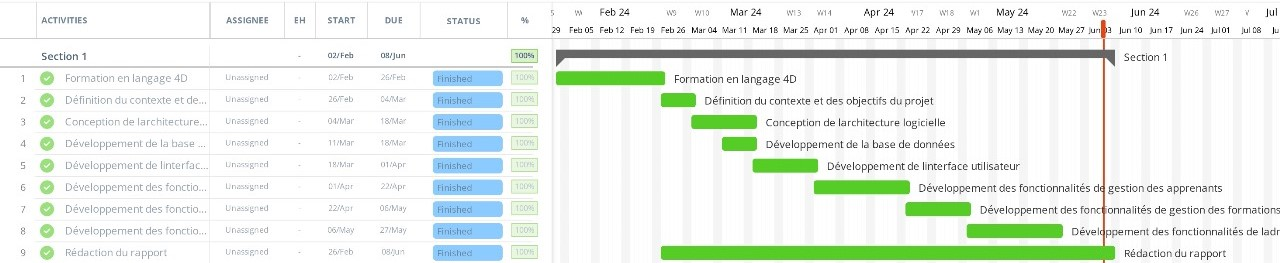
\includegraphics[width=18cm]{Figures/DiagrammeDeGantt.jpg}
%     \caption{Diagramme de Gantt.}
% \end{figure}

\begin{sidewaysfigure}
    \centering
    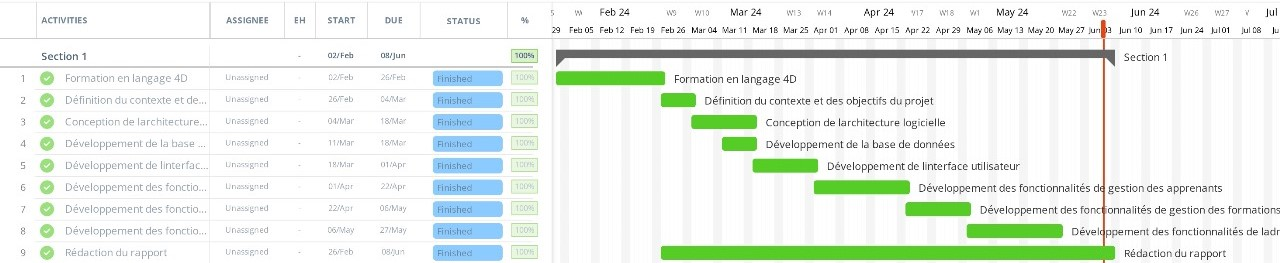
\includegraphics[width=\textheight,height=\textwidth,keepaspectratio]{Figures/DiagrammeDeGantt.jpg}
    \caption{Diagramme de Gantt.}
\end{sidewaysfigure}

\newpage
\subsection{Outils de collaboration:}

\subsubsection{Skype}

\begin{figure}[h]
    \centering
    
\includegraphics[scale=0.02]{Logos/Skype-Logo.png} % Replace with the actual filename of the IBM logo image
    \caption{Skype Logo}
\end{figure}

Skype est un logiciel propriétaire qui permet aux utilisateurs de passer des appels téléphoniques ou vidéo via Internet, ainsi que le partage d'écran. Les appels d’utilisateur à utilisateur sont gratuits, tandis que ceux vers les lignes téléphoniques fixes et les téléphones mobiles sont payants. Il existe des fonctionnalités additionnelles comme la messagerie instantanée, le transfert de fichiers et la visioconférence. 

Grâce à Skype, j'ai pu rester en contact régulier avec mon encadrant, mes collègues et les membres de l'entreprise. De plus, la fonction de partage d'écran de Skype a été extrêmement utile pour effectuer des présentations et des démonstrations de mon travail. Grâce à Skype, j'ai pu maintenir une communication fluide et efficace, ce qui a grandement contribué à la réussite de mon projet de fin d’étude.

\subsubsection{Git}

\begin{figure}[H]
    \centering
    
\includegraphics[scale=0.5]{Logos/git.png}
    \caption{Logo Git}
\end{figure}

Dans notre cas, et afin de conserver nos différentes versions du code source, nous avons
choisi de travailler avec Git comme logiciel de gestion de versions.

Git est un logiciel libre qui appartient au domaine publique (Licence GNU) et qui a
actuellement une communauté englobant près de 96\% des développeurs à travers le monde.

\subsubsection{GitLab}


\begin{figure}[H]
    \centering
    
\includegraphics[scale=0.1]{Logos/gitlab.jpg}
    \caption{Logo GitLab}
\end{figure}

Nous avons aussi opté pour GitLab, une plate-forme d'hébergement de code pour le
contrôle de version et la collaboration. Il permet, à nous et à d'autres, de travailler ensemble sur
des projets où que nous soyons.

\begin{figure}[H]
    \centering
    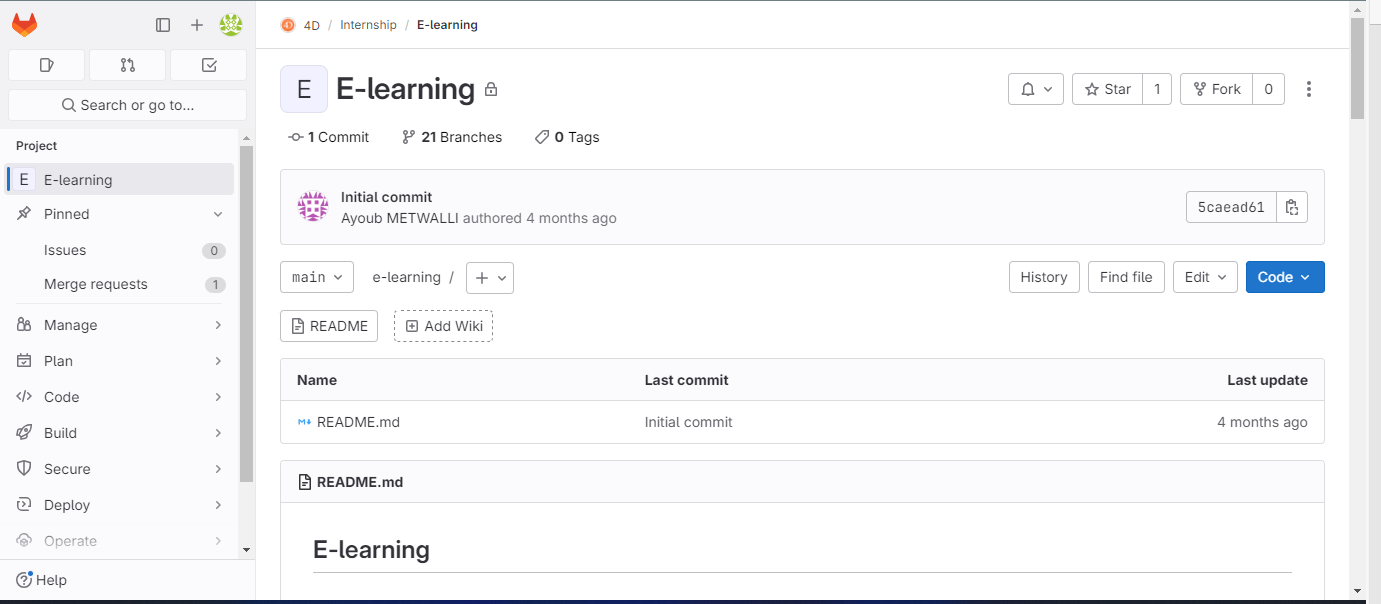
\includegraphics[width=19cm]{Figures/apercu.png}
    \caption{Aperçu globale de l'espace GitLab}
\end{figure}
\newpage

\section*{Conclusion}
Au cours de ce chapitre, nous avons mis l’accent sur le périmètre de notre projet. Nous avons éclairé
la méthodologie et le planning suivis pour mener ce projet. Nous entamerons dans le chapitre suivant
la phase d’analyse et spécification du système à développer au cours de laquelle nous comprenons en
profondeurs les besoins utilisateurs et construisons ainsi un système qui y répond.

